В данной главе рассмотрена архитектура генеративно-состязательной нейронной сети MuseGAN. Данная модель может использоваться для генерации с нуля и для продолжения композиции.

\section{ПРЕДСТАВЛЕНИЕ ДАННЫХ}

    В статье предлагается использовать представление в виде фортепианного ролла (рисунок \ref{fig:midi}) с несколькими дорожками \cite{musegan}. На данном рисунке горизонтальная прямая представляет собой время, а вертикальная -- высоту ноту (от меньшей к большей). Чёрный пиксель значит, что определённая нота сыграна в данный временной промежуток. Данная нейронная сеть моделирует полифоническую музыку с несколькими дорожками.
    
    \begin{figure}
        \centering
        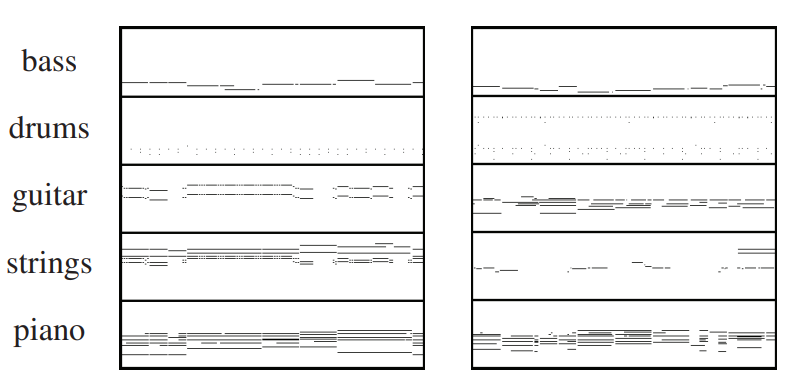
\includegraphics[scale=0.7]{tex/png/midi-example.png}
        \caption{Пример композиции с 5-ю дорожками \cite{musegan}}
        \label{fig:midi}
    \end{figure}
    
    
    Представление в виде фортепианного ролла — это бинарная матрица, отражающая наличие нот на различных временных шагах. 
    Горизонтальная ось — время, вертикальная ось — высота ноты (от низких к высоким). 
    При иллюстрации данной матрицы черный пиксель показывает, что определенная нота звучит на конкретном временном шаге. 
    Говоря формальным языком, фортепианный ролл с $\mathbf{M}$ дорожками одного такта представляется как тензор $ \mathbf{x} \in {0,1}^{R \times S \times M}$, где $ \mathbf{R} $ и $ \mathbf{S} $ обозначают число временных шагов в такте и число кандидатов в ноты соответственно. 
    Фортепианный ролл с $ \mathbf{M} $ дорожками из $ \mathbf{T} $ тактов представляется как $ \vec{x} = \{\vec{x}^{(t)}\}^T _ {t=1} $, где $ \vec{x}^{(t)} \in {0,1}^{R \times S \times M} $ обозначение фортепианного ролла с несколькими дорожками такта $ t $.
    
    Стоит заметить, что фортепианный ролл каждых такта и дорожки, как и для настоящих, так и для сгенерированных данных, представлен в виде матрицы фиксированного размера, что позволяет использовать сверточные нейронные сети.

\section{МОДЕЛИРОВАНИЕ НЕЗАВИСИМОСТИ ДОРОЖЕК}

    Существуют два стандартных способа создания музыки; рассмотрим их далее.
    \begin{enumerate}  
    \item Группа музыкантов, играющая на различных инструментах, может создавать музыку с помощью импровизации без подготовки и соглашений. Данный процесс известен как джем-сешн.
    \item Предоставление услуг композитора, который может выстроить композицию, обладая знаниями о гармонической структуре и доступном инструментарии. Далее музыканты могут сыграть уже сочиненную музыку.
    \end{enumerate}
    
    В архитектуре MuseGAN используется одновременно 3 модели, соответствующих этим композиционным подходам.
    
    Джем-модель (рисунок \ref{fig:jam}) устроена следующим образом: несколько генераторов работают независимо и создают музыку для собственных дорожек из приватного случайного вектора $\vec{z}_i $, $i=1,2,...,M$, где $M$ -- число дорожек. Эти генераторы получают обратную связь (через обратное распространение ошибки) от различных дискриминаторов.
    
    \begin{figure}
        \centering
        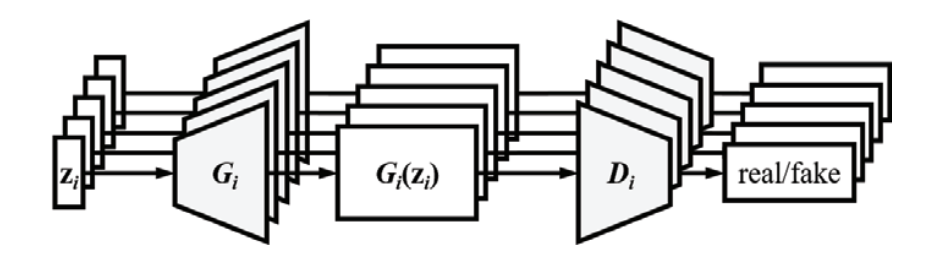
\includegraphics[scale=0.4]{tex/png/jamm.png}
        \caption{Представление джем-модели \cite{musegan}}
        \label{fig:jam}
    \end{figure}
    
    Модель-композитор (рисунок \ref{fig:composer}) включает в себя один генератор, который создает многоканальный фортепианный ролл, где каждый канал представляет определенную дорожку. 
    Данная модель требует только один общий случайный вектор $z$ (который может быть интерпретирован как замысел композитора) и один дискриминатор, который проверяет все $M$ вместе для того, чтобы определить, является ли вход настоящим или поддельным.
    
    \begin{figure}[h]
        \centering
        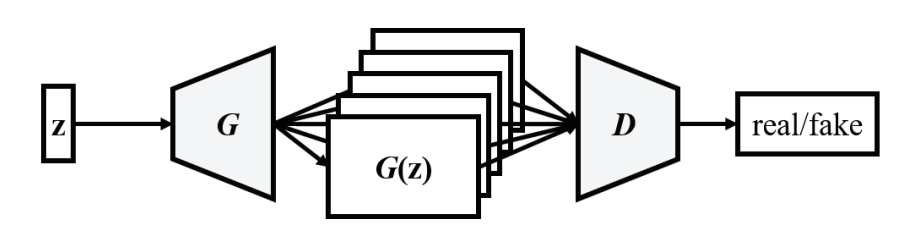
\includegraphics[scale=0.4]{tex/png/composer.png}
        \caption{Представление модели композитора \cite{musegan}}
        \label{fig:composer}
    \end{figure}
    
    При объединении идей джем-модели и модели композитора получается гибридная модель (рисунок \ref{fig:hybrid}). Каждый из $M$ генераторов принимает на вход “внутренний” случайный вектор $z$ и “внешний” случайный вектор. Роль “внутреннего” случайного вектора заключается в координации генераторов, как это делает композитор с музыкантами. Более того, только один дискриминатор оценивает все $M$ дорожек.
    
    \begin{figure}
        \centering
        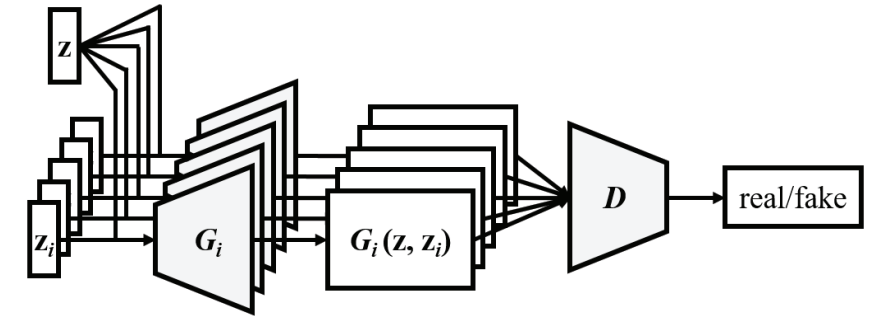
\includegraphics[scale=0.4]{tex/png/hybrid.png}
        \caption{Представление гибридной модели \cite{musegan}}
        \label{fig:hybrid}
    \end{figure}
    
    Главное отличие между моделью-композитором и гибридной — это гибкость. В гибридной модели можно использовать различные архитектуры нейронных сетей (т.е. варьировать число слоев, размер фильтра) и неодинаковые входы для каждого из генераторов. Таким образом, можно, например, менять процесс генерации одной определенной дорожки без потери связи между ними.

\section{МОДЕЛИРОВАНИЕ ВРЕМЕННОЙ СТРУКТУРЫ}
    Результатом генерирования описанных выше моделей является композиция с несколькими дорожками без согласованности между тактами. Для решения данной проблемы необходима временная модель для генерации музыки длиной в несколько тактов.
    
    Первый метод нацелен на генерацию музыкальных фраз фиксированной длины, что 
    достигается путем просмотра последовательности тактов. Генератор (рисунок \ref{fig:model_architecture}) состоит из двух частей: генератора временной структуры $G_{temp}$ и генератора тактов $G_{bar}$.
    
    \begin{figure}[h]
        \centering
        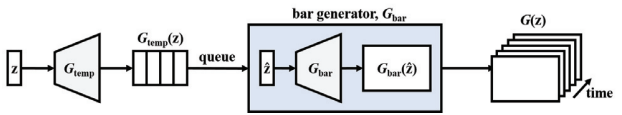
\includegraphics[scale=0.7]{tex/png/architecture_from_stratch.png}
        \caption{Архитектура модели для учёта временной структуры \cite{musegan}}
        \label{fig:model_architecture}
    \end{figure}
    
    $G_{temp}$ отображает вектор шума $z$ в некоторую последовательность латентных векторов $\vec{z} = \{ \vec{z}^{(t)} \} ^ T _ {t=1}$. Результирующий вектор (он несёт в себе временную информацию) затем использует $G_{bar}$ для последовательной генерации фортепианных роллов (такт за тактом):
    $$ G(z) = \{ G_{bar} \} ^ T _ {t=1}. $$
    
    Второй метод предполагает, что последовательность тактов $\vec{y}$ одной определённой дорожки задаётся человеком, и пытается выучить лежащую в основе временную структуру и генерировать оставшиеся дорожки. Зависимый от других дорожек генератор $G^{o}$ создает такты один за другим с помощью условного генератора тактов $G^o_{bar}$. Фортепианные роллы оставшихся дорожек такта $t$ генерируются $G^o_{bar}$, который принимает на вход условие $\vec{y}$ и зависящий от времени случайный шум ${\vec{z}} ^ {(t)}$.
    
    Для достижения такой условной генерации при работе с ситуациями большой размерности обучается энкодер $E$ для отображения $\vec{y}^{(t)}$ в пространство $\vec{z}^{(t)}$. Итоговая процедура выглядит следующим образом:
    $$ G^o(\vec{z}, \vec{y}) = \{G^o_{bar}(\vec{z}^{(t)}, E(\vec{y}^{(t)}))\}^T_{(t=1)}. $$
    
    Кодировщик будет извлекать “внутренние” признаки вместо “внешних”, т.к. “внешняя” дорожка не особо полезна для генерации остальных дорожек.

\section{АРХИТЕКТУРА МОДЕЛИ}
    
    MuseGAN представляет собой объединение и расширение представленных выше моделей (рисунок \ref{fig:full_musegan}). Рассмотрим более подробно данную архитектуру. 
    
    \begin{figure}[h]
        \centering
        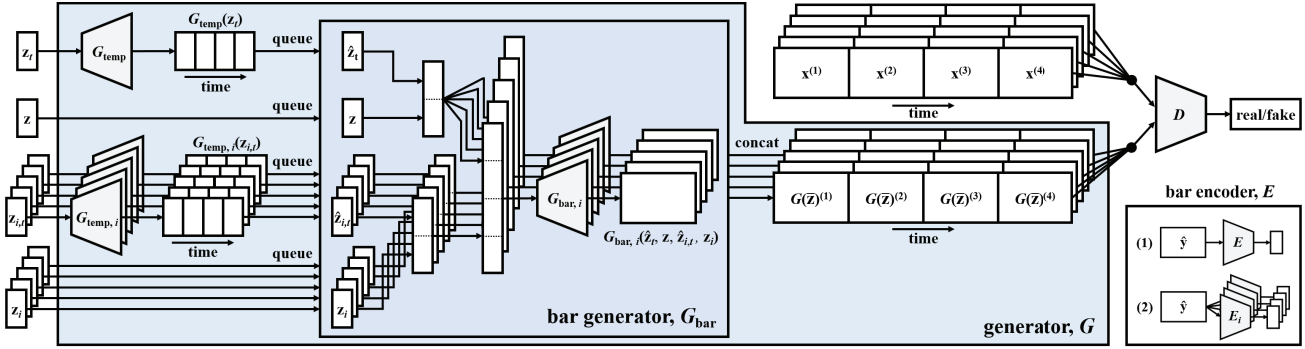
\includegraphics[scale=0.38]{tex/png/full_musegan.png}
        \caption{Полная архитектура модели генератора MuseGAN \cite{musegan}}
        \label{fig:full_musegan}
    \end{figure}
    
    Вход ($\vec{z}$) состоит из четырёх частей: 'внутренние'  независящие от времени случайные векторы $z$, 'внешние'  зависящие от времени векторы $z_i$, 'внутренние'  зависящие от времени случайные векторы $z_t$ и 'внешние'  зависящие от времени случайные векторы ${z_{i,t}}$. Для $i$-й дорожки ($i$ = 1,2, … , $M$), общий генератор временной структуры $G_{temp}$ и приватный генератор временной структуры $G_{temp, i}$ принимают на вход зависящие от времени случайные вектора $z_{t}$ и $z_{i,t}$ соответственно, и каждый из генераторов производит ряд из латентных векторов, содержащих “внутреннюю” и “внешнюю” временную информацию. Полученные ряды конкатенируют и поступают на вход генератору тактов, который последовательно создает фортепианные роллы. Процедуру генерации можно описать следующей формулой:
    $$G(\vec{z}) = \{G_{bar,i} (z, G_{temp}(z_{t})^{(t)}, z_{i}, G_{temp,i}(z_{i,t})^{(t)}) \} ^ {M,T} _ {i,t=1},$$
    где $G$ и $D$ реализованы как глубокие сверточные сети. $G$ прежде всего наращивает длительность ноты, а затем увеличивает высоту ноты, в то время как $D$ делает наоборот.
    
\section{ОЦЕНКА РАБОТЫ МОДЕЛИ}
    Для оценки работы модели можно использовать следующие метрики:
    \begin{enumerate}
        \item Количество пустых тактов к количеству всех тактов (в процентах).
        \item Количество используемых нот на такт (от 0 до 12).
        \item Количество правильных нот (в процентах). Правильной нотой считается та нота, которая не короче трёх временных шагов (то есть 32-ая нота). Данная метрика показывает как сильно композиция в результате фрагментирована.
        \item Ритмический паттерн: коэффициент нот, которые удовлетворяют 8-ми или 16-ти нотным паттернам, как обычно бывает в рок-композициях с размером 4/4.
        \item Тональное расстояние \cite{tonal-distance}. Оно измеряет гармоничность между парой тактов. Чем больше эта метрика, тем меньше композиция согласуется с собой.
    \end{enumerate}
    
    Для того, чтобы оценить итоговую модель -- считается статистика по данным значениям на реальных данных и потом они сравниваются с теми, которые посчитаны на данных, которые выдаёт генератор. В течении тренировки генератор должен создавать композиции, всё больше сближаясь к тренировочным данным.
    
    Недостатки модели были выявлены и описаны в главе исследований.